% Neutrino physics
% Target length: 30 pages

\graphicspath{{NeutrinoPhysics/Figs/}}

\chapter{Neutrino Physics}\label{chap:NeutrinoPhysics}

Neutrino physics will be discussed! \\
\\
-- Theory\\
-- Experiments\\
-- Future Experiments\\
\\
It may make sense to discuss the experiments as we go along...\\
\\
I think the chapter will work best with both past, present and future woven together.\\
And no distinct separation between theory and experiment (this is an experimental thesis after all...).\\
Can discuss the `neutrino problems' to motivate the theory of neutrino oscillations, and include the SNO and Kamiokande results within.\\
Then something similar with mass.\\
And as we get onto unanswered questions, can weave the propsed experiments into this.\\
I feel a section on the technology and concept of LAr TPCs will fit nicely into this setup.\\

%----------------------------------------------------------------------------------------------------------------------------------------------------------------------------
\section{Neutrino Theory}\label{sec:NeutrinoTheory}

\subsection{Neutrino Oscillations}\label{sec:NeutrinoOscillations}

Derive 2-flavour case.\\
Extend to 3 flavour.\\
Discuss CP violation.\\

\subsection{Neutrino Mass}\label{sec:NeutrinoMass}

Mass hierarchy.\\
Absolute mass.\\


%----------------------------------------------------------------------------------------------------------------------------------------------------------------------------
\section{Future Neutrino Experiments}\label{sec:FutureNeutrinoExperiments}

%----------------------------------------------------------------------------------------------------------------------------------------------------------------------------
\section{The LAr TPC Concept}\label{sec:LArTPC}

The use of a liquid argon time projection chamber (LArTPC) as a high-precision fine-grained detector medium holds much promise for the successful resolution of the open questions in neutrino physics.  A great amount of R\&D work has taken place to advance the maturity of the technology and pioneering experiments, such as ICARUS \cite{ICARUS2004}, have further increased the understanding of the neutrino community of the detector techniques.  Past and currently running experiments at Fermilab, such as ArgoNeuT [], LArIAT [] and MicroBooNE [], are successfully using LArTPCs to take and analyse data and it seems certain to be the future of neutrino physics in the U.S.

This section will provide a brief history of LArTPC technology and motivate its potential when used in a huge experiment such as DUNE.  The basic operation of such a detector will also be described to provide background for discussion of the DUNE and 35t experiments, and of reconstruction in LArTPCs, in future chapters.

\subsection{A Brief History of Time (Projection Chambers)}\label{sec:LArTPCHistory}

The use of a time projection chamber as a potential particle detector was put forward by David Nygren in 1974 \cite{Nygren1974}.  He envisioned bubble-chamber quality data but with the possiblity of digital readout of the data, fascilitating extremely fine spatial resolution, good timing resolution and fast recovery after triggering.  The basic concept is a drift chamber containing a noble gas placed within a field to drift ionisation electrons created by a propagating particle towards a multielectron array.  This setup allows full three-dimensional reconstruction by combining information from the two-dimensional readout plane with the drift time.  Nygren also included a magnetic field to assist particle identification in his design, shown in Fig. \ref{fig:NygrenTPC}.

\begin{figure}[ht]
  \centering
  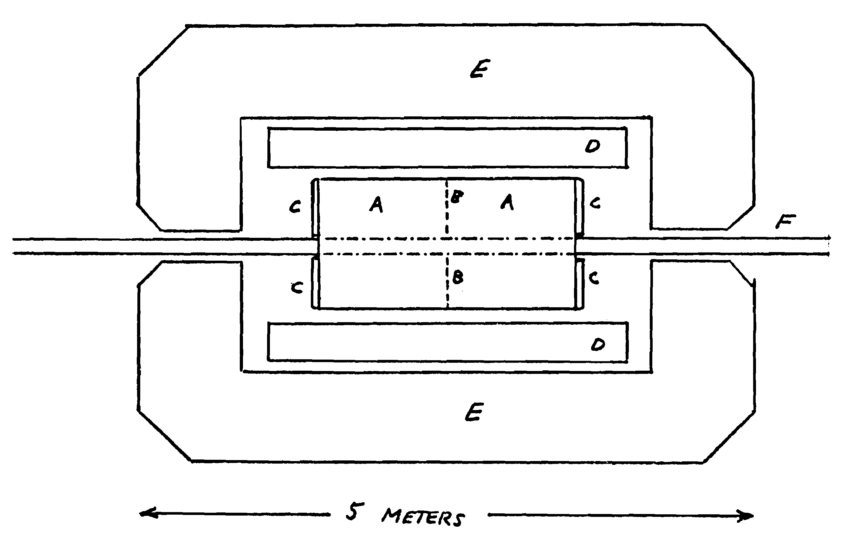
\includegraphics[width=10cm]{NygrenTPC.png}
  \caption[Original TPC design, Nygren (1974)]{The original concept of the time projection chamber particle detector, drawn by David Nygren in 1974 \cite{Nygren1974}.}
  \label{fig:NygrenTPC}
\end{figure}

The extension of this concept to a liquid argon TPC and it potential as a high-precision fine-grained detector medium in neutrino physics was proposed by Carlo Rubbia in 1977 \cite{Rubbia1977}.  The use of a noble liquid rather than gas is necessary in neutrino experiments to provide a high enough target mass to increase the probability of a neutrino interaction.  Noble liquids have high electron mobility and low diffusion, favourable properties as the detection of particles is from the ionisation and scintillation light created by the particles.  Given the necessity of a high electric field in order to drift these electrons to the readout places, excellent dielectric properties are also required; noble liquids possess such qualities.  The properties of liquid argon which make it almost perfect for this use are demonstrated in the table in Table \ref{tab:NobleProperties}.

\begin{table}[ht]
  \caption{Properties of noble elements relevant when considering a TPC medium for a neutrino experiment.}
  \label{tab:NobleProperties}
  \centering
  \begin{tabular}{ m{5cm} || m{1.5cm} | m{1.5cm} | m{1.5cm} | m{1.5cm} | m{1.5cm} | m{1.5cm} }
     & Water & He & Ne & \color{red} Ar & Kr & Xe \\
    \hline\hline
    Boiling point [K] @ 1 atm & 373 & 4.2 & 27.1 & \color{red} 87.3 & 120.0 & 165.0 \\
    \hline
    Density [g/cm$^3$] & 1 & 0.125 & 1.2 & \color{red} 1.4 & 2.4 & 3.0 \\
    \hline
    Radiation length [cm] & 36.1 & 755.2 & 24.0 & \color{red} 14.0 & 4.9 & 2.8 \\
    \hline
    Scintillation [$\gamma$/MeV] & - & 19 000 & 30 000 & \color{red} 40 000 & 25 000 & 42 000 \\
    \hline
    dE/dx [MeV/cm] & 1.9 & & 1.4 & \color{red} 2.1 & 3.0 & 3.8 \\
    \hline
    Scintillation $\lambda$ [nm] & & 80 & 78 & \color{red} 128 & 150 & 175 \\
    \hline
    Natural abundance (Earth atm) [ppm] & & 5.2 & 18.2 & \color{red} 9340.0 & 1.10 & 0.09 \\
    \hline
    Electron mobility [cm$^2$/Vs] & & low & low & \color{red} 400 & 1200 & 2200 \\
    \hline\hline
  \end{tabular}
\end{table}

An additional advantage of this technology is the low threshold for detection; this is set by the ionisation threshold of liquid argon and is only $23.6 \pm 0.5$ eV [].  Rubbia realised that a LArTPC could be the digital replacement for the high quality particle detection methods used in bubble chambers, very common in neutrino physics in the 1970s.  He proposed the first LArTPC detector design, shown in Fig. \ref{fig:RubbiaLArTPC}, which bears a striking resemblense to the LArTPC used in experiments today.

\begin{figure}[ht]
  \centering
  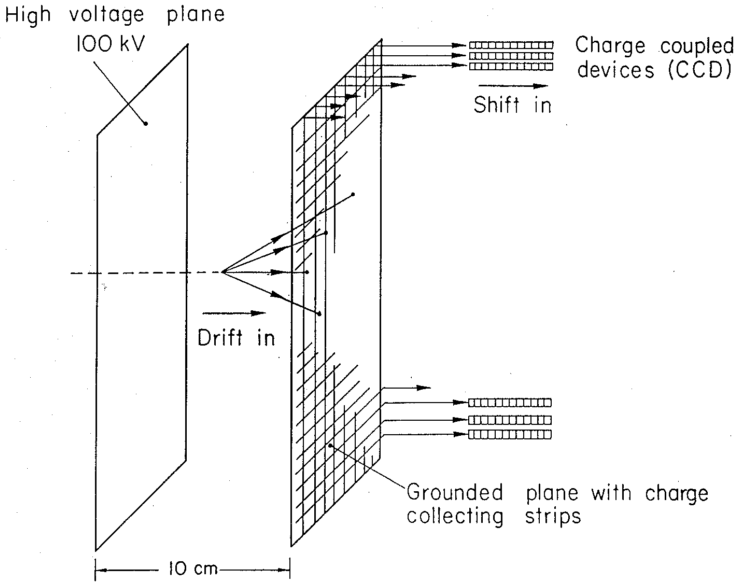
\includegraphics[width=10cm]{RubbiaLArTPC.png}
  \caption[First LArTPC detector, Rubbia (1977)]{The LArTPC detector proposed by Carlo Rubbia in 1977 \cite{Rubbia1977}.}
  \label{fig:RubbiaLArTPC}
\end{figure}

Constructing and operating such a detector was beyond the technology of the time, and is still being understood today.  The operation of a LArTPC detector and the challenges associated with this are the subject of section \ref{sec:LArTPCOperation}.

\subsection{LAr TPC Operation}\label{sec:LArTPCOperation}

explain how they work

new subsubsection

[FIND OR MAKE A FIGURE TO GO WITH THE FOLLOWING DESCRIPTION...]

A LArTPC typically consists of a single, or multiple anode and cathode, at either end of an active drift region.  An ionising particle passing through a LArTPC causes electrons to become free from argon atoms and, in the presence of a field, drift towards an anode where they are read out.

The readout consists of multiple wires planes with different orientations to facilitate the reconstruction.  The wires are either `induction' wires, which allow the electrons to deposit charge but continue past, or `collection' wires, on which the electric field lines end and all the charge on the electron is collected.  Each wire plane is therefore held at a different `bias voltage' to prevent any field lines ending on the induction wire, thus creating local electric fields which promote the continuing forward motion of the electrons.  The signal seen is therefore dependent on the type of wire plane; a bipolar pulse on an induction plane wire and unipolar on a collection plane wire.  It is also common, though not essential, to make use of a `grid plane' upstream of the signal planes in order to shield them from the electron charge until they are close.  Without such a plane, the bipolar pulse would be highly asymmetric, though would still have zero integral.  It also makes changing the drift voltage (controlling the electric field) slightly easier as the signal planes are somewhat shielded from its effects.  MicroBooNE does not operate with a grid plane and, although the 35t and the DUNE reference design make use of a grid plane, it is uncertain whether the benefit outweighs the cost for a huge LArTPC detector such as the DUNE far detector.  It is worth mentioning alternative readout possibilities have been suggested but, given the scale of future LArTPCs, it is highly unlikely a viable solution which delivers superior readout at a comparable cost will be found.


Given the positive ions that are left in the medium, there is the possibility of recombination at a later time and therefore a loss of information about the initial interaction.


This is however accompanied by a flash of scintillation light which is hugely useful as a means of determining the event `start time' ($t_0$); without this information it would be impossible to place an absolute time scale on the interaction and we would therefore not be able to resolve the coordinate along the drift direction.  The magnitude of the electric field applied is the key to both processes and there is thus a compromise which must be struck in order to preserve as much information as possible.  The graph in Fig. \ref{fig:ElectricFieldScintillationIonisation} demonstrates this; a field of $500$ V/cm is often chosen in current LAr neutrino experiments.

\begin{figure}[ht]
  \centering
  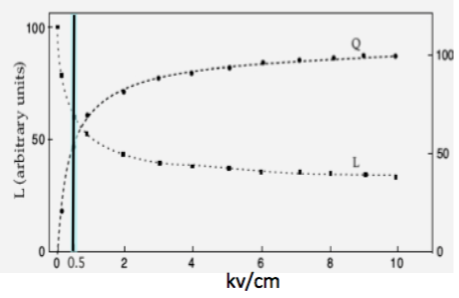
\includegraphics[width=12cm]{ElectricFieldScintillationIonisation.png}
  \caption[Affect of electric field on luminosity of ionisation electrons and scintillation light in a LArTPC]{Demonstration of the competing effect the electric field has on the luminosity of the ionisation electrons and scintillation light arriving at the detector readout.  Since both are essential in reconstructing the complete interactions, a balance must be found. [PLACEHOLDER IMAGE].}
  \label{fig:ElectronFieldScintiallationIonisation}
\end{figure}

A cathode is held at a high voltage



Flesh this stuff out...


U plane, V plane and collection all held at different fields.  Slightly increasing in order to promote forward motion of the electrons.  V held at 0V because it's cheaper (don't need crazy voltages, just some negative (still quite high, ~100V), 0V and some positive.
Grid plane (also held at potential) is to sheild the APAs from the electrons until they are close.  Not needed, but if not present then pulse wouldn't be very bipolar! The charge in both portions will still equate but the leading end will be muchhhh longer.  All electric field lines (generated from movement of electrons) end on the cathode; don't want them to end on the induction wires (hence making sure the field increases).  We want them to end on the collection planes, which collects the charge.  Signal shaping time (along with gain, the two front-end ASIC parameters) is to let the charge leave the wire before being hit again (or something like this!).  Deconvolution I still need to understand...


In 35t, we have FE ASICs which are the very front end and apply the signal shaping and gain.  Have regulators to control the power these receive (these are noisy...).  Also ADC ASICs to do digitisation in the cold.  MicroBooNE don't do this, this just have the front end and do everything else in the warm.  FE ASICs are the problem, same for uBooNE and 35t.  ADC ASIC has stuck code problem.
